\chapter{Attivit\`a Sperimentale}
\definecolor{mygreen}{rgb}{0.0.33, 0.42, 0.18}
Questo capitolo rappresenta la parte sperimentale del lavoro di Tesi.\\*
Nel seguito si illustrano gli esperimenti di \emph{fault injection} condotti sul sistema nell'ambiente descritto nel capitolo 4, e si discutono i risultati ottenuti.\\*
La traccia ferrotramviaria scelta per l'analisi \`e un sottoinsieme della linea \texttt{T1} della Tramvia di Firenze, che si estende per $4.25044$ chilometri dal terminal di \emph{Villa Costanza}, nel comune di Scandicci. 
\begin{figure}[h]
	\centering
	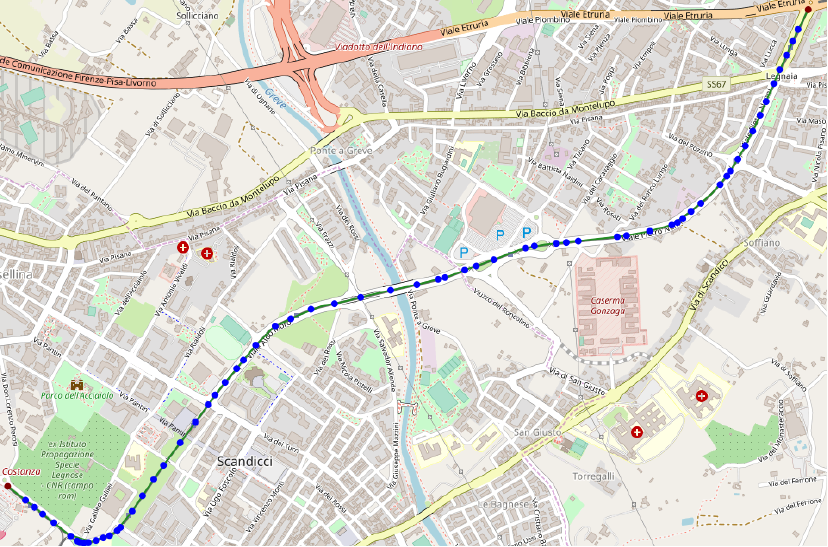
\includegraphics[width=0.7\linewidth]{img/itrace}
	\caption{Traccia di analisi}
	\label{fig:linea-test}
\end{figure}
\section{Misure di interesse}
La \emph{fault tolerance} del sistema verr\`a valutata in termini degli errori che SFA commette nella stima delle seguenti grandezze:
\begin{itemize}
	\item Posizione del treno, espressa in coordinate ECEF;
	\item Velocit\`a del treno, proiettata sui tre assi cartesiani.
\end{itemize}
ECEF \`e l'acronimo di \emph{Earth Centered Earth Fixed}. Una coordinata ECEF esprime la posizione di un oggetto immerso in un sistema di riferimento cartesiano a 3 dimensioni, con origine nel centro della Terra.
\section{Guasti iniettati}
In relazione al \emph{fault model} individuato al capitolo 4, sono stati iniettati i seguenti guasti:
\begin{enumerate}
	\item[(1)] Soppressione del canale di comunicazione tra IMU e SFA;
	\item[(2)] Alterazione del contenuto dei messaggi trasmessi dai sensori al modulo SFA;
	\item[(3)] Sopressione del canale di comunicazione tra Odometro e SFA.
\end{enumerate}
Rispetto al sistema reale descritto nel capitolo 3, i guasti (1) e (3) simulano un guasto hardware nei bus dati che collegano i sensori alla scheda \emph{NVidia TX-Jetson} o comunque l'interruzione del funzionamento dei sensori, sia essa permanente o temporanea.\\*
Il guasto (2) simula un comportamento di \texttt{UDP} comunque preventivabile, data la natura \emph{best effort} del protocollo.\\*Quando si utilizza \texttt{UDP} \`e opportuno non fare mai assunzioni riguardo il corretto ordinamento e l'integrit\`a dei messaggi trasmessi.\\*
\section{Esperimenti}
Durante l'attivit\`a di analisi sono stati effettuati numerosi esperimenti. In questa sezione, si riportano in dettaglio solo i risultati ritenuti pi\`u interessanti, mentre i rimanenti vengono descritti a un livello pi\`u generico.\\*
La soppressione del canale di comunicazione tra IMU e modulo SFA, quando protratta per un periodo superiore a $5$ secondi, ha prodotto un'interruzione del servizio. Questo \`e in linea con le aspettative in quanto IMU \`e il sensore principale su cui si basa l'esecuzione di SFA, e senza di esso l'algoritmo non pu\`o funzionare.\\*
Il valore limite di $5$ secondi trova giustificazione andando a osservare l'implementazione del modulo SFA. Quest'ultimo infatti \`e programmato in maniera tale che il massimo numero di campionamenti IMU che pu\`o predire attraverso regressione lineare \`e $500$.\\*
La frequenza di campionamento di IMU \`e pari a:
$$100\;Hz\;=\;100\; \frac{\mbox{campionamenti}}{\mbox{s}}$$ Pertanto:
$$
\frac{500 \mbox{ campionamenti}}{100\frac{ \mbox{  campionamenti}}{\mbox{s}}} = \frac{500}{100}\mbox{ s} = 5\mbox{ s}
$$
L'alterazione del contenuto dei messaggi non ha portato a effetti rilevabili, a condizione che il software abbia maturato una adeguata esperienza circa il comportamento corretto dei sensori, ovvero, abbia stimato correttamente i parametri del modello di regressione attraverso il quale vengono predette le misure mancanti.\\*
Nel seguito di questa sezione, si discutono gli esperimenti (3).\\*
Per ciascuna grandezza osservata viene riportato il valore medio, il valore
massimo e la deviazione standard (dev. std.) dell'errore commesso da SFA nel relativo processo di stima.
\subsection{Golden Run}
Per ottenere un termine di paragone consistente, il sistema viene eseguito prima senza l'iniezione di guasti.\\*
I risultati ottenuti durante la campagna di \emph{fault injection} verranno quindi valutati in relazione ai risultati ottenuti dal software senza introduzione di guasti. Questa prima esecuzione del software prende il nome di \emph{golden run}.
\begin{table}[h]
	\centering
	\begin{tabular}{|p{3.25cm}|p{2cm}|p{2cm}|p{2cm}|p{2cm}|}
		\hline 
		\textbf{Sensori integrati} & \textbf{Frequenza IMU}  & \textbf{Frequenza odometro} & \textbf{Varianza Odometro} & \textbf{Iterazioni} \\ 
		\hline 
		IMU, Odometro & 100 Hz & 10 Hz & 0.0004 & 10 \\
		\hline 
	\end{tabular}
	\caption{Golden Run: workload}
	\label{tab:exp12}
\end{table}
\begin{table}[h]
	\centering
	\begin{tabular}{|p{2cm}|p{3cm}|p{3cm}|p{3cm}|}
		\hline 
		\textbf{Misura} & \textbf{Errore medio}  & \textbf{Errore massimo} & \textbf{Dev. std. errore}\\ 
		\hline 
		ECEF X & 3.5826 m & 20.1141 m & 5.60308 m \\ 
		\hline 
		ECEF Y & 0.0243133 m & 0.362813 m & 0.0452763 m \\ 
		\hline 
		ECEF Z & 3.56432e-06 m & 3.19201e-06 m & 8.81543e-06 m \\ 
		\hline 
		Velocit\`a X & 0.0169528 m/s & 0.124472 m/s & 0.0199173 m/s \\ 
		\hline 
		Velocit\`a Y & 0.0394826 m/s & 0.847261 m/s & 0.0828195 m/s \\ 
		\hline 
		Velocit\`a Z & 0.00382241 m/s & 0.0192343 m/s & 0.00314704 m/s \\ 
		\hline 
	\end{tabular}
	\caption{Golden Run: Risultati}
	\label{tab:exp12res}
\end{table}
\FloatBarrier
\subsection{Soppressione della comunicazione odometro - SFA}
In questo scenario il \emph{faultload} consiste nella soppressione del canale di comunicazione tra Odometro e modulo SFA.
\subsubsection{Esperimento 3.1}
Si sopprime il canale di comunicazione \textbf{per tutta la durata dell'esperimento}.\\*
\begin{table}[h]
	\centering
	\begin{tabular}{|p{3.25cm}|p{2cm}|p{2cm}|p{2cm}|p{2cm}|}
		\hline 
		\textbf{Sensori integrati} & \textbf{Frequenza IMU}  & \textbf{Frequenza odometro} & \textbf{Varianza Odometro} & \textbf{Iterazioni} \\ 
		\hline 
		IMU, Odometro & 100 Hz & 10 Hz & 0.0004 & 10 \\
		\hline 
	\end{tabular}
	\caption{Esperimento 3.1: workload}
\end{table}
	\begin{table}[h]
	\centering
	\begin{tabular}{|p{2cm}|p{3cm}|p{3cm}|p{3cm}|}
		\hline 
		\textbf{Misura} & \textbf{Errore medio}  & \textbf{Errore massimo} & \textbf{Dev. std. errore}\\ 
		\hline 
		ECEF X & 861.883 m & 2431.1 m & 678.953 m \\ 
		\hline 
		ECEF Y & 348.814 m & 1518.65 m & 499.222 m \\ 
		\hline 
		ECEF Z & 0.123305 m & 0.155086 m & 0.567656 m \\ 
		\hline 
		Velocit\`a X & 8.20331 m/s & 30.782 m/s & 7.32822 m/s \\ 
		\hline 
		Velocit\`a Y & 23.4213 m/s & 75.1929 m/s & 20.0333 m/s \\ 
		\hline 
		Velocit\`a Z & 87.7399 m/s & 87.1907 m/s & 245.723 m/s \\ 
		\hline 
	\end{tabular}
	\caption{Esperimento 3.1: Risultati}
	\label{tab:exp11res}
\end{table}
\begin{table}[h]
	\centering
	\begin{tabular}{|p{2cm}|p{3.2cm}|p{3cm}|p{3cm}|}
		\hline 
		\textbf{Misura} 
		& \textbf{Errore medio} 
		& \textbf{Errore massimo}
		& \textbf{Dev. std. errore}\\ 
		\hline 
		ECEF X & \textcolor{red}{\textbf{+23957.5 \%}}& \textcolor{red}{\textbf{+11986.5 \%}} & \textcolor{red}{\textbf{+12017.5 \%}}  \\ 
		\hline 
		ECEF Y & \textcolor{red}{\textbf{+1.43456e+06 \%}}& \textcolor{red}{\textbf{+4.18477e+05 \%}} & \textcolor{red}{\textbf{+1.10251e+06 \%}}  \\ 
		\hline 
		ECEF Z & \textcolor{red}{\textbf{+3.45933e+06 \%}}& \textcolor{red}{\textbf{+1.77827e+06 \%}} & \textcolor{red}{\textbf{+1.75916e+06 \%}}  \\ 
		\hline 
		Velocit\`a X & \textcolor{red}{\textbf{+48289.1 \%}}& \textcolor{red}{\textbf{+24630.1 \%}} & \textcolor{red}{\textbf{+36693.2 \%}}  \\ 
		\hline 
		Velocit\`a Y & \textcolor{red}{\textbf{+59220.6 \%}}& \textcolor{red}{\textbf{+8774.82 \%}} & \textcolor{red}{\textbf{+24089.1 \%}}  \\ 
		\hline 
		Velocit\`a Z & \textcolor{red}{\textbf{+2.29531e+06 \%}}& \textcolor{red}{\textbf{+1.27743e+06 \%}}& \textcolor{red}{\textbf{+2.77046e+06 \%}} \\ 
		\hline 
	\end{tabular} 
	\caption{Esperimento 3.1: Confronto con Golden Run} 
\end{table}
\begin{figure}[h]
	\centering
	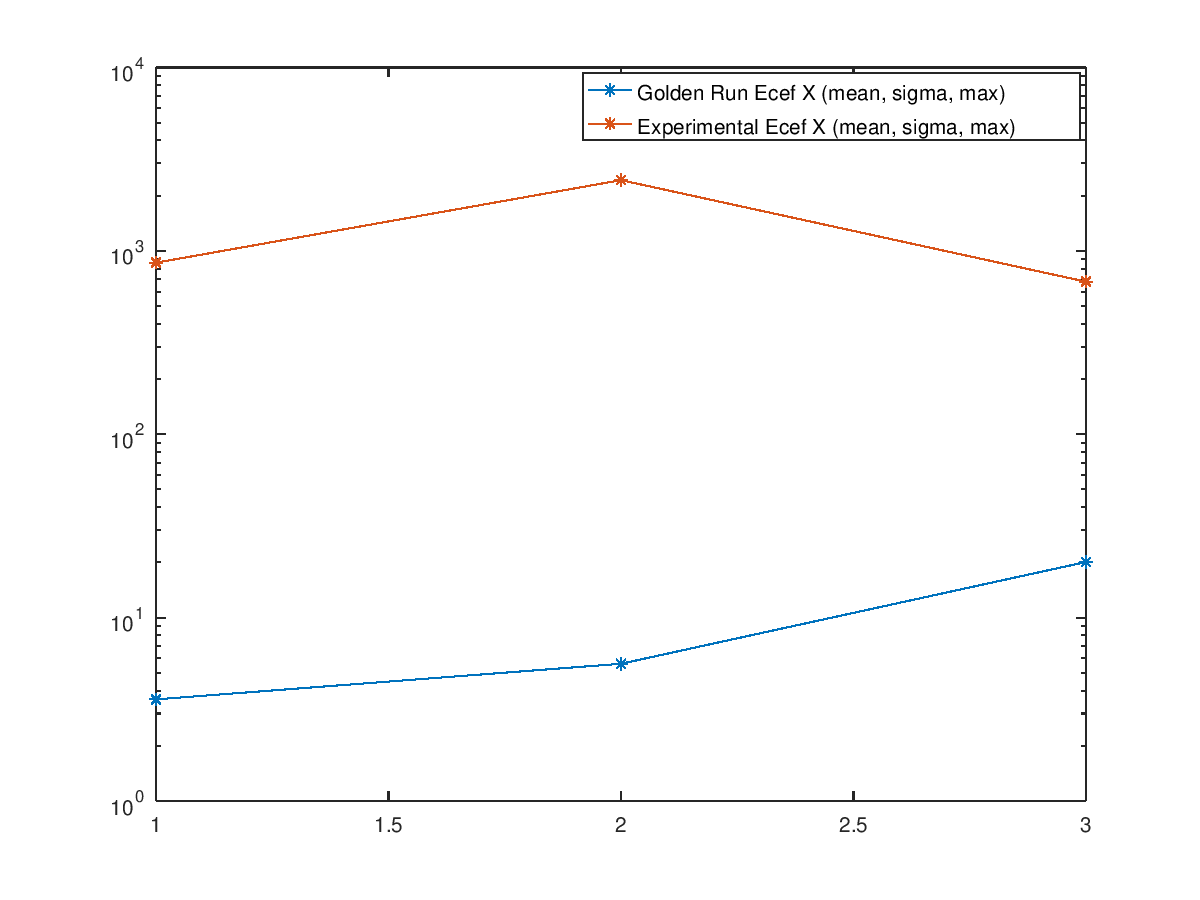
\includegraphics[width=0.7\linewidth]{img/exp11plot}
	\caption{Esperimento 3.1: Grafico di confronto ECEF X con Golden Run}
	\label{fig:exp11plot}
\end{figure}
\begin{figure}[h]
	\centering
	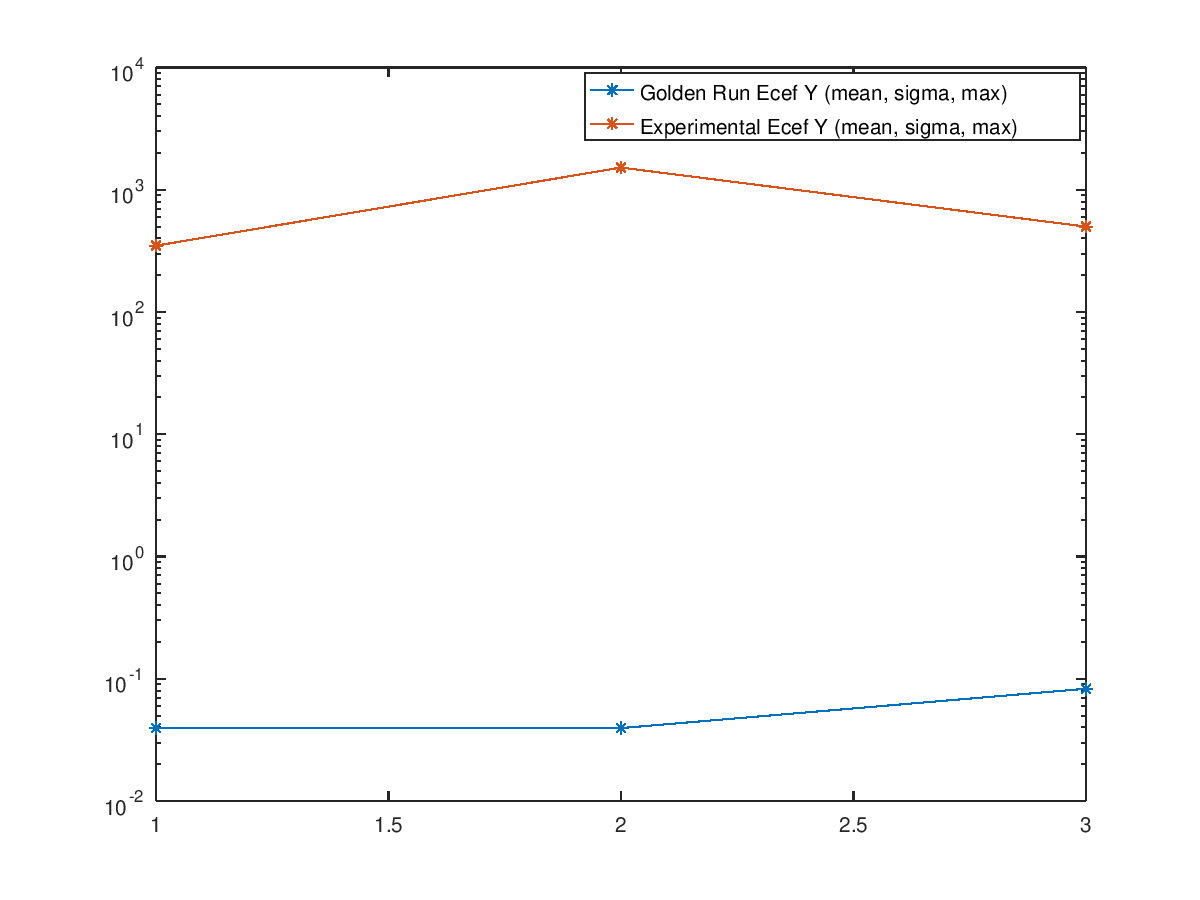
\includegraphics[width=0.7\linewidth]{img/exp11ecefY}
	\caption{Esperimento 3.1: Grafico di confronto ECEF Y con Golden Run}
\end{figure}
\begin{figure}[h]
	\centering
	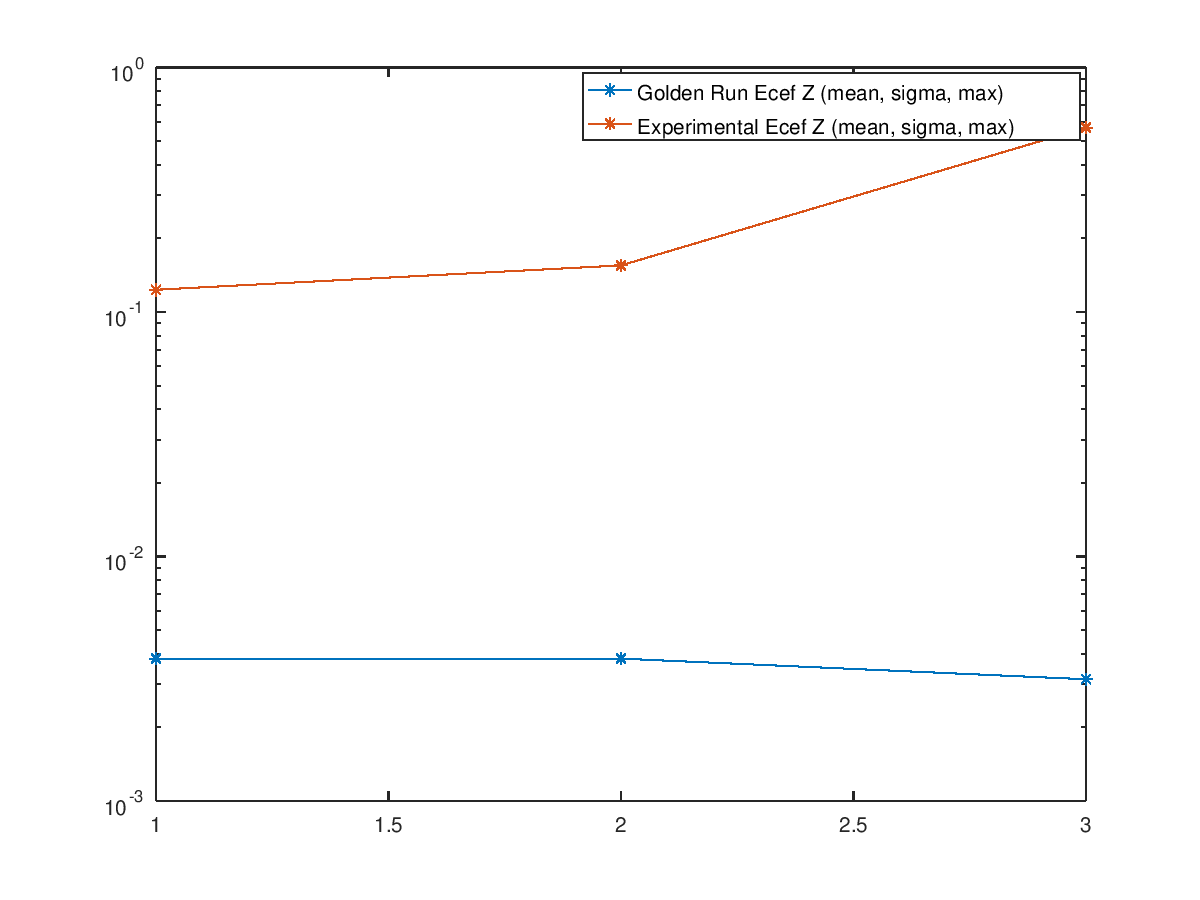
\includegraphics[width=0.7\linewidth]{img/exp11ecefZ}
	\caption{Esperimento 3.1: Grafico di confronto ECEF Z con Golden Run}
\end{figure}
\FloatBarrier
Alimentare SFA utilizzando esclusivamente le misurazioni di IMU conduce a una netta divergenza dell'errore, sia in termini di posizione che in termini di velocit\`a.\\*
Questi risultati non sono accettabili. In questa fattispecie, tuttavia, \`e stato iniettato un importante \emph{faultload} altamente improbabile da osservare sul campo.
\subsubsection{Esperimento 3.2}
Si sopprime il canale di comunicazione tra SFA e Odometro durante \textbf{la prima met\`a della simulazione}.\\*
\begin{table}[h]
	\centering
\begin{tabular}{|p{3.25cm}|p{2cm}|p{2cm}|p{2cm}|p{2cm}|}
	\hline 
	\textbf{Sensori integrati} & \textbf{Frequenza IMU}  & \textbf{Frequenza odometro} & \textbf{Varianza Odometro} & \textbf{Iterazioni} \\ 
	\hline 
	IMU, Odometro & 100 Hz & 10 Hz & 0.0004 & 10 \\
	\hline 
\end{tabular}
	\caption{Esperimento 3.2: workload}
\end{table}
\begin{table}[h]
	\centering
	\begin{tabular}{|p{2cm}|p{3.2cm}|p{3cm}|p{3cm}|}
		\hline 
		\textbf{Misura} 
		& \textbf{Errore medio} 
		& \textbf{Errore massimo}
		& \textbf{Dev. std. errore}\\ 
		\hline 
		ECEF X & 4.3248 m & 20.5617 m & 5.41018 m \\ 
		\hline 
		ECEF Y & 0.0226056 m & 0.39742 m & 0.04816 m \\ 
		\hline 
		ECEF Z & 3.81041e-06 m & 3.30294e-05 m & 9.04865e-06 m \\ 
		\hline 
		Velocit\`a X & 0.0248871 m/s & 0.150687 m/s & 0.0260141 m/s \\ 
		\hline 
		Velocit\`a Y & 0.0475246 m/s & 0.908185 m/s & 0.0899591 m/s \\ 
		\hline 
		Velocit\`a Z & 0.00406042 m/s & 0.0228906 m/s & 0.00340827 m/s \\ 
		\hline 
	\end{tabular} 
	\caption{Esperimento 3.2: Risultati}
\end{table}
\begin{table}[h]
	\centering
	\begin{tabular}{|p{2cm}|p{3.2cm}|p{3cm}|p{3cm}|}
		\hline 
		\textbf{Misura} 
		& \textbf{Errore medio} 
		& \textbf{Errore massimo}
		& \textbf{Dev. std. errore}\\ 
		\hline 
		ECEF X & \textcolor{red}{\textbf{+20.7168 \%}}& \textcolor{red}{\textbf{+2.22531 \%}} & \textcolor{mygreen}{\textbf{-3.44275 \%}}  \\ 
		\hline 
		ECEF Y & \textcolor{mygreen}{\textbf{-7.02373 \%}}& \textcolor{red}{\textbf{+9.53852 \%}} & \textcolor{red}{\textbf{+6.36912 \%}}  \\ 
		\hline 
		ECEF Z & \textcolor{red}{\textbf{+6.90426 \%}}& \textcolor{red}{\textbf{+3.47524 \%}} & \textcolor{red}{\textbf{+2.64559 \%}}  \\ 
		\hline 
		Velocit\`a X & \textcolor{red}{\textbf{+46.8023 \%}}& \textcolor{red}{\textbf{+21.061 \%}} & \textcolor{red}{\textbf{+30.6106 \%}}  \\ 
		\hline 
		Velocit\`a Y & \textcolor{red}{\textbf{+20.3685 \%}}& \textcolor{red}{\textbf{+7.1907 \%}} & \textcolor{red}{\textbf{+8.62068 \%}}  \\ 
		\hline 
		Velocit\`a Z & \textcolor{red}{\textbf{+6.2267 \%}}& \textcolor{red}{\textbf{+19.0093 \%}}& \textcolor{red}{\textbf{+8.30082 \%}} \\ 
		\hline 
	\end{tabular} 
	\caption{Esperimento 3.2: Confronto con golden run} 
\end{table}
\begin{figure}[h]
	\centering
	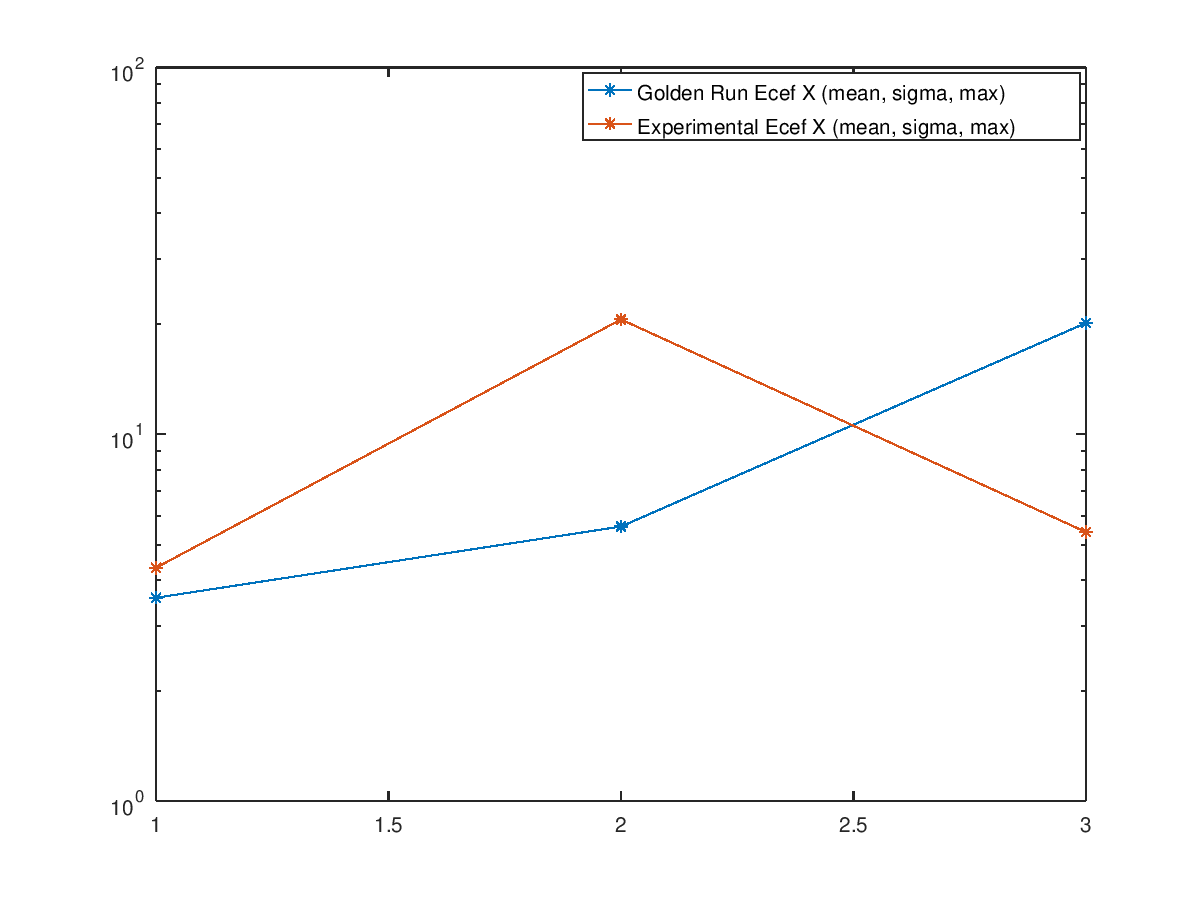
\includegraphics[width=0.7\linewidth]{img/exp12plot}
	\caption{Esperimento 3.2: Grafico di confronto ECEF X con Golden Run}
\end{figure}
\begin{figure}[h]
	\centering
	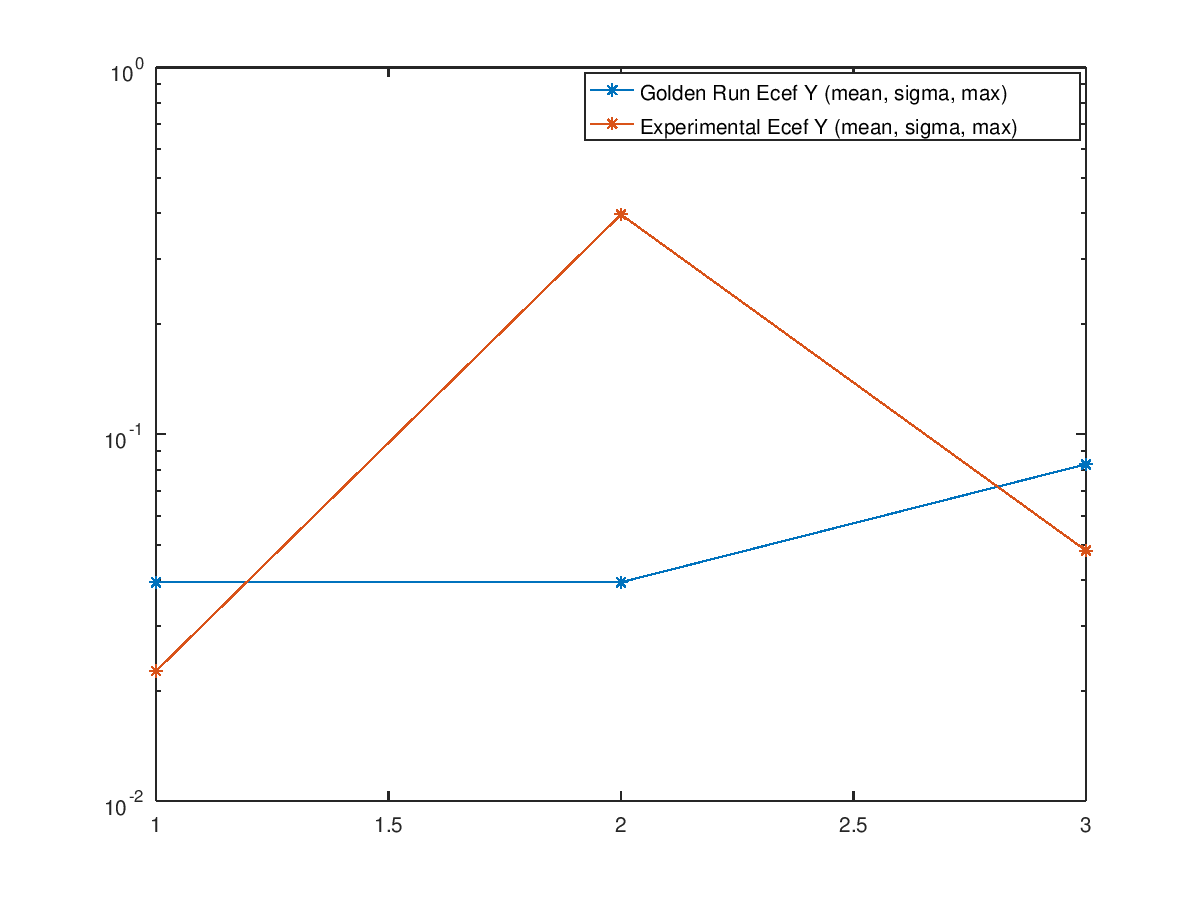
\includegraphics[width=0.7\linewidth]{img/exp12ecefY}
	\caption{Esperimento 3.2: Grafico di confronto ECEF Y con Golden Run}
\end{figure}
\begin{figure}[h]
	\centering
	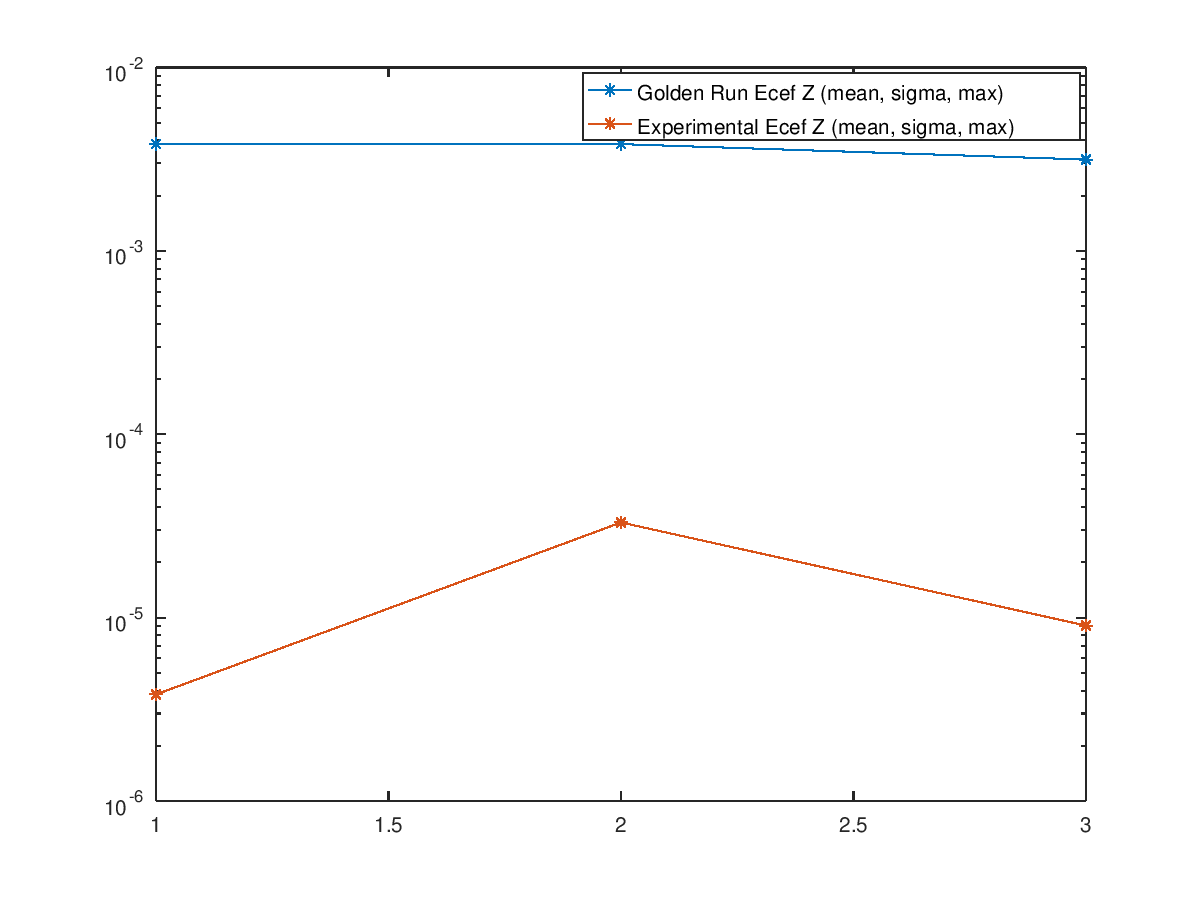
\includegraphics[width=0.7\linewidth]{img/exp12ecefZ}
	\caption{Esperimento 3.2: Grafico di confronto ECEF Z con Golden Run}
\end{figure}
\FloatBarrier
Si osserva un lieve degrado delle performance che influisce in maniera non particolarmente significativa ai fini del posizionamento.\\*
La grandezza che appare pi\`u degradata \`e la velocit\`a, e questo permane in linea con le aspettative, poich\`e l'odometro \`e il sensore preposto a fornire le misure di velocit\`a al sistema.
\subsubsection{Esperimento 3.3}
Si sopprime il canale di comunicazione tra SFA e Odometro durante \textbf{la seconda met\`a della simulazione}.\\* 
\begin{table}[h]
	\centering
\begin{tabular}{|p{3.25cm}|p{2cm}|p{2cm}|p{2cm}|p{2cm}|}
	\hline 
	\textbf{Sensori integrati} & \textbf{Frequenza IMU}  & \textbf{Frequenza odometro} & \textbf{Varianza Odometro} & \textbf{Iterazioni} \\ 
	\hline 
	IMU, Odometro & 100 Hz & 10 Hz & 0.0004 & 10 \\
	\hline 
\end{tabular}
	\caption{Esperimento 3.3: workload}
\end{table}
\begin{table}[h]
	\centering
	\begin{tabular}{|p{2cm}|p{3.2cm}|p{3cm}|p{3cm}|}
	\hline 
	\textbf{Misura} 
	& \textbf{Errore medio} 
	& \textbf{Errore massimo}
	& \textbf{Dev. std. errore}\\ 
	\hline 
	ECEF X & 3.57373 m & 20.1609 m & 5.60304 m \\ 
	\hline 
	ECEF Y & 0.0234386 m & 0.366496 m & 0.0445943 m \\ 
	\hline 
	ECEF Z & 3.55578e-06 m & 3.19863e-05 m & 8.7636e-06 m \\ 
	\hline 
	Velocit\`a X & 0.0184494 m/s & 0.129497 m/s & 0.0222426 m/s \\ 
	\hline 
	Velocit\`a Y & 0.0396467 m/s & 0.863711 m/s & 0.084737 m/s \\ 
	\hline 
	Velocit\`a Z & 0.00355928 m/s & 0.0189619 m/s & 0.00306268 m/s \\ 
	\hline 
\end{tabular} 
	\caption{Esperimento 3.3: Risultati}
\end{table}
\begin{table}[h]
	\centering
	\begin{tabular}{|p{2cm}|p{3.2cm}|p{3cm}|p{3cm}|}
	\hline 
	\textbf{Misura} 
	& \textbf{Errore medio} 
	& \textbf{Errore massimo}
	& \textbf{Dev. std. errore}\\ 
	\hline 
	ECEF X & \textcolor{mygreen}{\textbf{-0.247586 \%}}& \textcolor{red}{\textbf{+0.232673 \%}} & \textcolor{mygreen}{\textbf{-0.000714 \%}}  \\ 
	\hline 
	ECEF Y & \textcolor{mygreen}{\textbf{-3.59762 \%}}& \textcolor{red}{\textbf{+1.01512 \%}} & \textcolor{mygreen}{\textbf{-1.50631 \%}}  \\ 
	\hline 
	ECEF Z & \textcolor{mygreen}{\textbf{-0.239597 \%}}& \textcolor{red}{\textbf{+0.207393 \%}} & \textcolor{mygreen}{\textbf{-0.587946 \%}}  \\ 
	\hline 
	Velocit\`a X & \textcolor{red}{\textbf{+8.82804 \%}}& \textcolor{red}{\textbf{+4.03705 \%}} & \textcolor{red}{\textbf{+11.6748 \%}}  \\ 
	\hline 
	Velocit\`a Y & \textcolor{red}{\textbf{+0.415626 \%}}& \textcolor{red}{\textbf{+1.94155 \%}} & \textcolor{red}{\textbf{+2.31528 \%}}  \\ 
	\hline 
	Velocit\`a Z & \textcolor{mygreen}{\textbf{-6.88388 \%}}& \textcolor{mygreen}{\textbf{-1.41622 \%}}& \textcolor{mygreen}{\textbf{-2.68061 \%}} \\ 
	\hline 
\end{tabular} 
	\caption{Esperimento 3.3: Confronto con golden run} 
\end{table}
\begin{figure}[h]
	\centering
	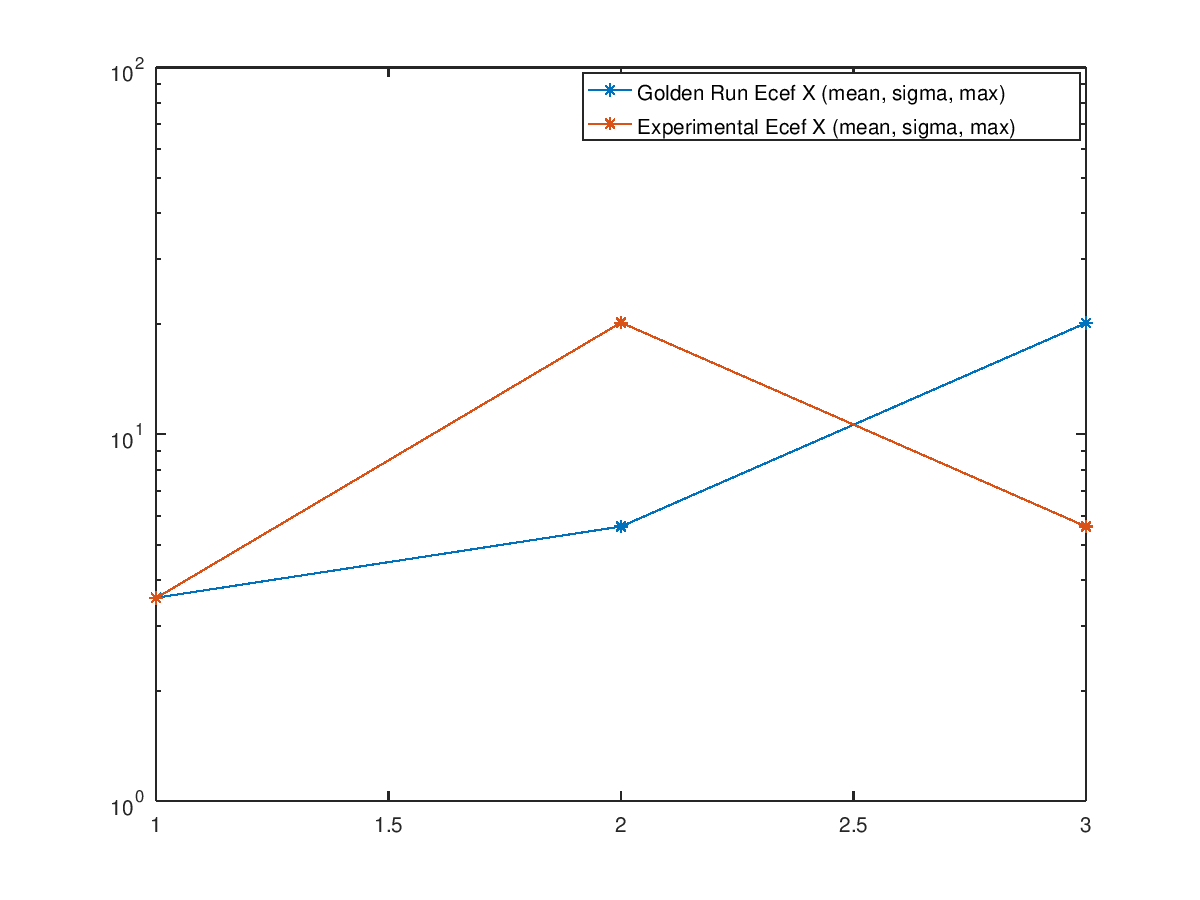
\includegraphics[width=0.7\linewidth]{img/exp13plot}
	\caption{Esperimento 3.3: Grafico di confronto ECEF X con Golden Run}
	\label{fig:exp13plot}
\end{figure}
\begin{figure}[h]
	\centering
	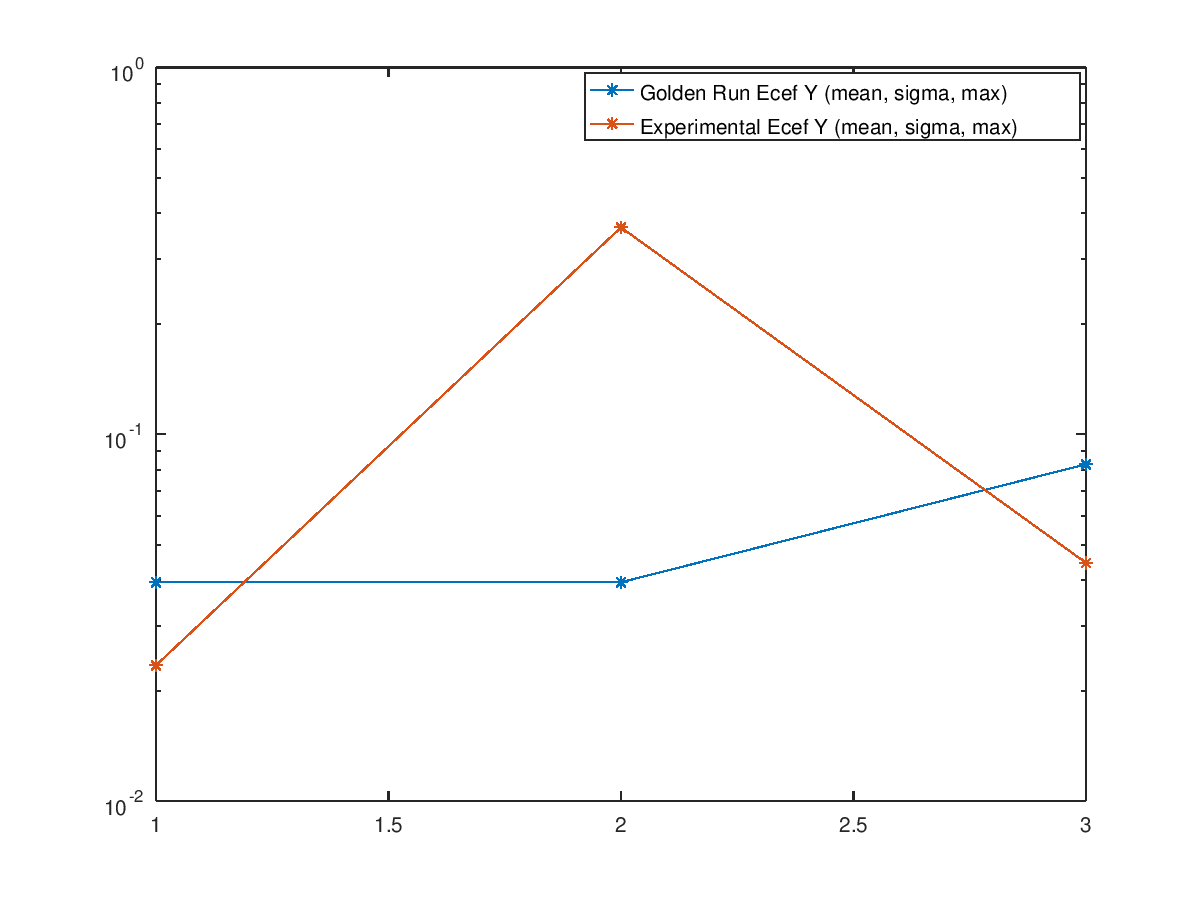
\includegraphics[width=0.7\linewidth]{img/exp13ecefY}
	\caption{Esperimento 3.3: Grafico di confronto ECEF Y con Golden Run}
\end{figure}
\begin{figure}[h]
	\centering
	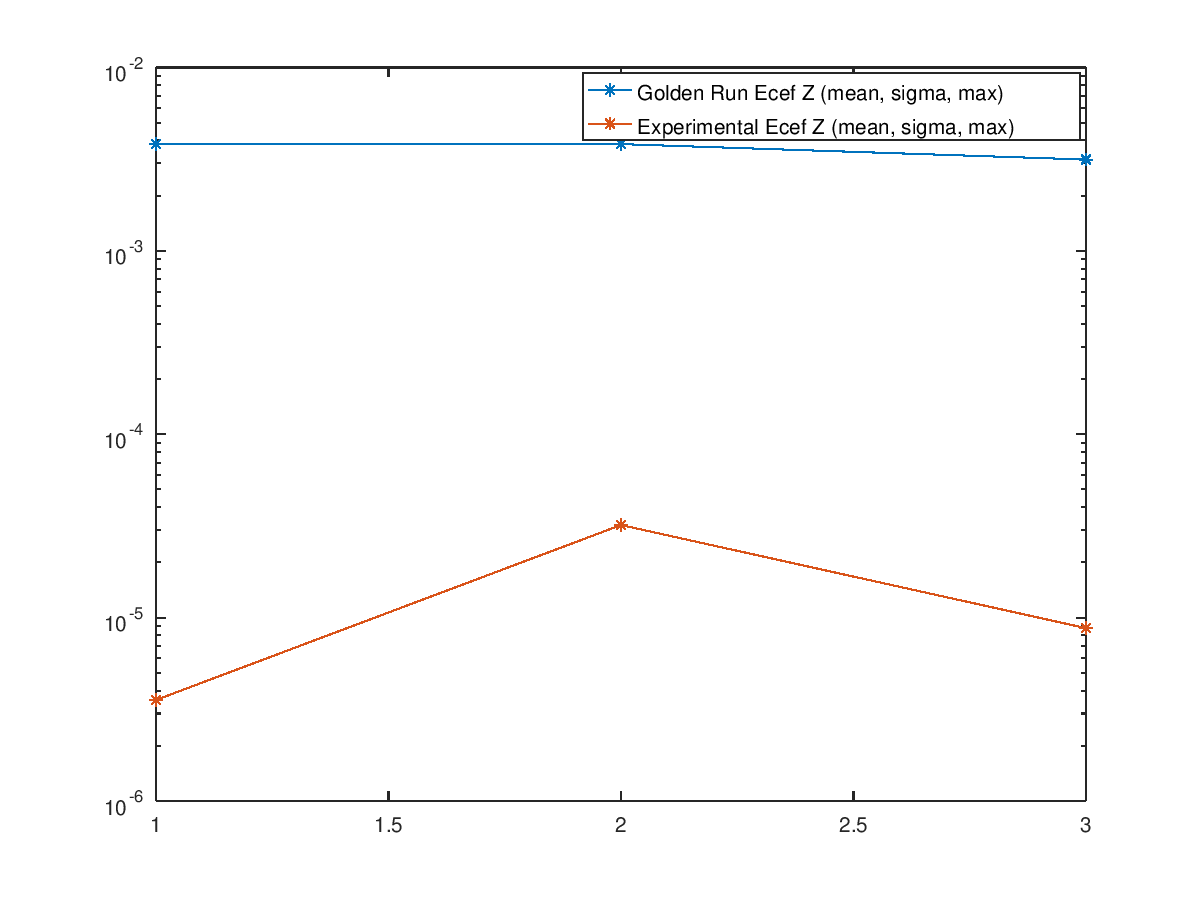
\includegraphics[width=0.7\linewidth]{img/exp13ecefZ}
	\caption{Esperimento 3.3: Grafico di confronto ECEF Z con Golden Run}
\end{figure}
\FloatBarrier
Non si osservano particolari variazioni rispetto ai risultati ottenuti nella \emph{golden run}. \`E ragionevole ipotizzare che la causa di questo comportamento sia da ricercare nella sezione di traccia in cui si \`e soppresso il canale di comunicazione tra Odometro e SFA. Nella prima met\`a la traccia compie una curva netta, mentre nella seconda essa si sviluppa in modo approssimativamente lineare.
\FloatBarrier
\section{Considerazioni finali}
La campagna di \emph{fault injection} effettuata sul modulo SFA ha condotto alle conclusioni che seguono:
\begin{itemize}
	\item Il sistema \`e in grado di tollerare la perdita di misure IMU fino a un massimo di 5 secondi. Superata questa soglia, il sistema si blocca e smette di erogare il proprio servizio. Questa modalit\`a di fallimento \`e comunque facilmente rilevabile da OBCU, la quale potrebbe agire sul treno di conseguenza, ad esempio fermandolo. Si osserverebbe un degrado della qualit\`a del servizio offerto, ma si avrebbe comunque un fallimento \emph{safe}.
	\item Entro certi limiti di approssimazione, il sistema sembra tollerare bene la ricezione di messaggi fuori ordine o alterati. Infatti, attraverso un meccanismo di \emph{regressione lineare}, il sistema \`e in grado di riconoscere e scartare messaggi che hanno un'elevata probabilit\`a di contenere valori non affidabili. Un messaggio ricevuto fuori ordine \`e semplicemente un messaggio che ha probabilit\`a $1$ di non essere affidabile.\\*
	Quando un messaggio viene scartato, l'informazione mancante viene stimata e fornita al sistema come se fosse stata campionata dai sensori.
	\item L'odometro sembra particolarmente utile quando il movimento del treno \`e caratterizzato da repentini cambi di direzione, come nel caso di curve molto strette. Su tratti sufficientemente lineari, il sistema sembra comportarsi correttamente anche se viene alimentato esclusivamente dal sensore inerziale.
	\item Non \`e stato possibile osservare il sistema quando sottoposto a misure di tipo GPS, e le \emph{software probe} che sono state inserite all'interno del codice potrebbero aver degradato le performance, seppur trascurabilmente. Si ipotizza che l'aggiunta di un nuovo strumento di misura, come il GPS, possa migliorare le performance osservate.
	\item Quando la stima della posizione non diverge, \`e stato osservato che l'errore massimo sulla stima della posizione permane, in modulo, pari a circa 20 metri.
\end{itemize}